\documentclass[a4paper,10pt]{article}
\usepackage[utf8]{inputenc}
\usepackage{amsmath,amssymb}
\usepackage{enumerate}
\usepackage{ngerman}
%\usepackage{graphicx}
\usepackage{ifpdf}
\usepackage[usenames]{color}
\usepackage[left=2.5cm,right=2.5cm,top=2.5cm,bottom=2.5cm]{geometry}
\usepackage[titles]{tocloft}
\usepackage[colorlinks=true,linkcolor=black]{hyperref}
\usepackage[pdftex]{graphicx}
\usepackage{geometry}
%\geometry{top=0cm,bottom=0cm,left=0cm,right=0cm,nohead,nofoot}


\title{Validierung}
\date{}

\author{Usman Ghani Ahmed \\
Philip Caroli\\
Maximilian Madlung\\ 
Jeremias Mechler\\ 
Fabian Neundorf}

\ifpdf
\DeclareGraphicsExtensions{.png,.pdf}
\else
\DeclareGraphicsExtensions{.eps}
\fi

% Einrückung bei Absätzen
\setlength{\parindent}{0mm}
% Zeilenabstand bei Absätzen
\setlength{\parskip}{2mm}

\begin{document}
 
\vspace{5cm}
\maketitle
\begin{center}
\vspace{3cm}
\huge{Praxis der Softwareentwicklung \\
Gruppe 3 \\[0.5cm]
Entwicklung eines "`Monopoly"'-Ähnlichen Spiels \\[0.5cm]
%
\includegraphics[height=2cm]{kitlogo_de_rgb}  \\[0.5cm]
WS 2010 / 2011} \\[2cm]
%\textcolor{red}{! DRAFT !}
\end{center}

\newpage

\tableofcontents

\newpage

\section{Unit Tests}

\subsection{Testfälle und Testszenarien aus dem Pflichtenheft}

Folgende Funktionssequenzen sind in der grafischen Benutzeroberfläche getestet worden. Der Server wurde entsprechend mitgeprüft: \\
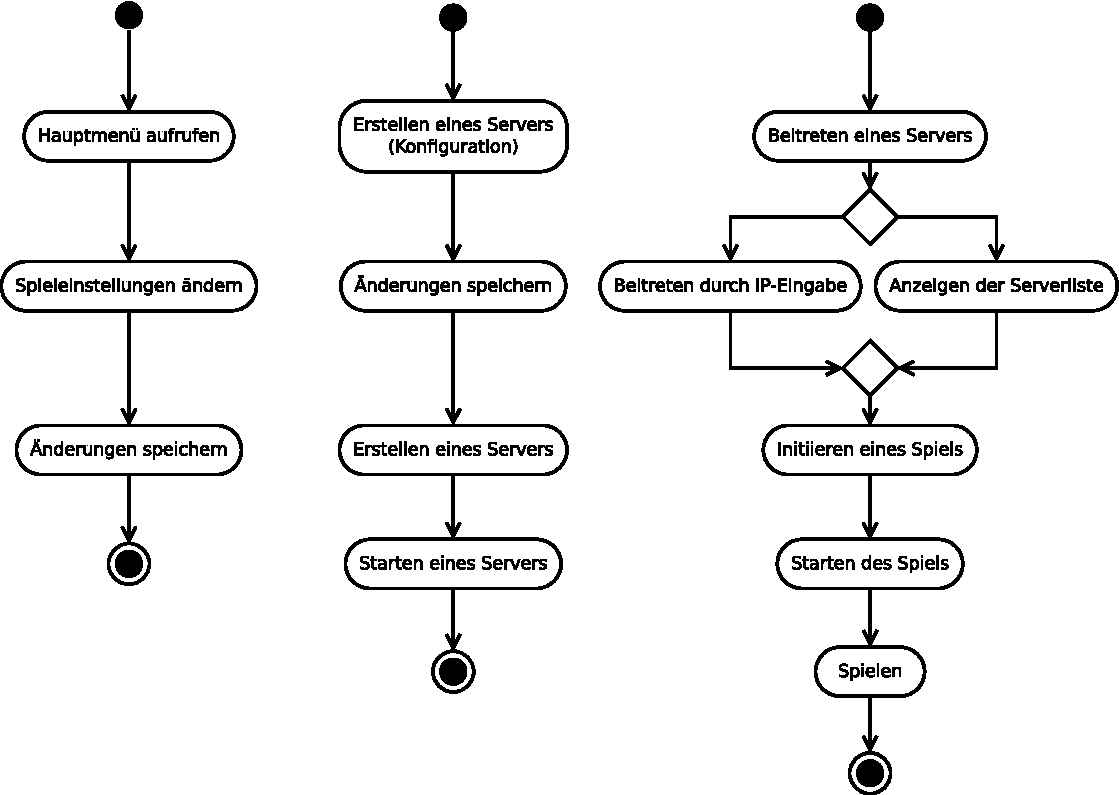
\includegraphics[width=17cm]{Diagram1} \\
Folgende Datenkonsistenzen sind eingehalten worden:
\begin{itemize}
\item Zu jedem Zeitpunkt muss ein Spielername definiert sein
\item Einstellungen können nur geladen werden, wenn die zu ladende Datei vollständig ist
\item Einstellungen können nur gespeichert werden, wenn alle Felder korrekt ausgefüllt sind
\item Der Zustand des Spielfeldes muss zwischen Client und Server identisch sein
\end{itemize}
Folgende unzulässigen Aktionen müssen korrent behandelt werden:
\begin{itemize}
\item Unzulässiges Übersenden von Kommandos an Client und Server (DoS)
\item Überschreitung der maximalen Teilnehmeranzahl
\item Belegung von Ressourcen durch häufiges Beitreten und Verlassen von Clients
\item Unerwarteter Verbindungsabbruch (Timeout, Connection Reset)
\item Reaktion auf Verbindungsverlust zum Server
\item Unsauberer Restart des Clients
\item Übersenden von undefinierten und unzulässigen Befehlen an Client und Server
\end{itemize}
\newpage
Interoperabilität, Usability:
\begin{itemize}
\item Richtige Funktion mit Client und Server der anderen Gruppe
\item Korrekte Darstellung auf verschiedenen Betriebssystemen (Windows, Linux, OS X)
\item Verschiedene Bildschirmauflösungen
\item nicht-standardmäßige Systemschriftgröße
\end{itemize}
Testszenarien:
\begin{itemize}
\item "`Erste Inbetriebnahme mit Starten eines Servers"' \\
Starten des Programms $\rightarrow$ im Hauptmenü "`Einstellungen"' aufrufen $\rightarrow$ Daten eingeben $\rightarrow$ "`Spieleinstellungen speichern"' anklicken $\rightarrow$ im Hauptmenü "`Spiel erstellen"' anklicken $\rightarrow$ Einstellungen vornehmen $\rightarrow$ "`Einstellungen speichern"' anklicken $\rightarrow$ "`Erstellen des Servers"' anklicken $\rightarrow$ "`Starten des Servers"' anklicken.
\item "`Einem Spiel beitreten (durch Serverliste), spielen und aufgeben"' \\
Starten des Programms $\rightarrow$ "`Spiel beitreten"' auswählen$\rightarrow$ "`Serverliste"' anklicken $\rightarrow$ Server auswählen $\rightarrow$ verbinden $\rightarrow$ Bereitschaft setzen $\rightarrow$ Würfeln, Spielzüge durchführen $\rightarrow$ aufgeben
\item "`Einzelspieler"' \\
"`Spiel erstellen"' anklicken $\rightarrow$ Mindest-Anzahl der Spieler $>1$ setzen, andere Einstellungen vornehmen $\rightarrow$ "`Einstellungen speichern"' anklicken $\rightarrow$ "`Erstellen des Servers"' anklicken $\rightarrow$ "`Starten des Servers"' anklicken.
\item "`Voller Server"' \\
Spieler versucht auf vollen Server zu verbinden $\rightarrow$ erhält Meldung, dass die maximale Teilnehmeranzahl erreicht ist
\item "`Serverabsturz"' \\
Mehrere Spieler spielen $\rightarrow$ Server stürzt ab $\rightarrow$ Server wird neu gestartet $\rightarrow$ Spiel wird über Sicherungs-Datei auf dem Server wiederhergestellt
\item "`Abwesenheit eines Spielers"' \\
Ein Spieler muss einen Zug vornehmen und reagiert eine bestimmte Zeit nicht $\rightarrow$ er wird zwangsweise aus dem Spiel entfernt $\rightarrow$ das Vermögen fällt der Bank zu
\end{itemize}


\section{Integrations- und Belastungstests}
\subsection{Testplan für die GUI}

Die Tests sind gegliedert in Aufgabe, Auffallend, Reaktion.
\begin{enumerate}
\item Wechseln der Sprache \\
Aufgabe: Öffnen aller Fenster in jedem Spielzustand und die Sprache auf alle 3 Sprachen umstellen\\

Auffallend:
1. Ohne Spiel: Das Join Gamefenster verändert seinen Text nicht. Create Game hat einen nichtübersetzten Text ""host"" Im Hilfetext fehlen nützliche Informationen.
2. Warteraum: Gleiches wie ohne Spiel, nur der Button "Send" im Chat bekommt erst mit dem Wechsel der Sprache einen Text.
3. Im Spiel: Keine neuen Bugs.

Reaktion:
Chat-Senden-Button gefixt, Join Gamefenster gefixt, Hostproblem gefixt, Hilfefenster mit HTML, Hilfetext im Deutschen aktualisiert

\item Verändern von Settings \\
Aufgabe: Verändern der Settings in jedem Spielzustand.\\

Auffallend: Vor dem Spiel: Name hat Auswirkung auf den Spielernamen, im Warteraum und Spiel ist es aber zu spät. Die Fenstergröße hat keine Auswirkung auf das Fenster.

Reaktion: Die Fenstergröße hat nun einen Einfluss darauf wie das Spiel beim nächsten Neustart aussieht. Außerdem wird eine Settingsfile nun sicher angelegt.

\item Erstellen eines Spiels \\
Aufgabe: Erstellen eines Spiels in jedem Spielzustand.\\

Auffallend: Während noch nichts gestartet ist ohne Probleme. Während des Warteraums alles Planmäßig verlaufen (Spielernamen der KI änderten sich). Während eines laufenden Spiels kommt es zu Problemen, durch den Readybutton scheinen die Knöpfe und andere Elemente des Spiels durch.

Reaktion: Wurde gefixt.
\item Erstellen eines Spiels (2) \\
Aufgabe: Erstellen eines Spiels mit ungültigen Parametern\\

Auffallend: Servername leer: Spiel erstellenknopf verharrt und wartet auf richtige Eingabe. 9 Spieler möglich, AI Player >= Insgesamt Player nicht möglich.

Reaktion: Spielerzahl insgesamt limitiert
\item Klicken auf Spielernamen \\
Aufgabe: Klicken auf die Spielernamen im Waiting Room sowie im Spiel\\

Auffallend: Im Warteraum kommt außer einem "Clicked on Player X" in der Konsole keine Reaktion.
Im Spiel öffnet sich ein Handelsfenster mit negativem Anfangsgeld und es ist möglich sich selbst anzuhandeln.

Reaktion: -1 Bug behoben, man kann nun nicht mehr mit sich selbst handeln.
\item Klicken auf Gefängnisfreikarte und Gefängnisfreigeld \\
Aufgabe: Klicken auf Gefängnisfreikarte und Gefängnisfreigeld während des Spiels: man ist nicht am Zug, man ist am Zug aber nicht im Gefängnis, ein Bot ist im Gefängnis aber man selbst nicht, man selbst ist im Gefängnis

Auffallend: Nicht am Zug: keine Reaktion außer in der Konsole dass es versucht wird, am Zug aber nicht im Gefängnis: keine Reaktion außer in der Konsole dass es versucht wird, Während die KI im Gefängnis ist ebenfalls keine Reaktion, Bei 6,5 Spielern kann die GUI sich aus dem Gefängnis frei kaufen.

Reaktion: Bis auf die Gefängnisfreikarte die noch nicht implementiert ist läuft es wie es sollte.
\item Klicken auf die Felder \\
Aufgabe: Auf alle Spielfelder klicken, auf eigene, ungekaufte, Felder der Mitspieler\\

Auffallend: Bei ungekauften Feldern wird eine Exception geworfen

Reaktion: Fehler behoben
\item Endturn\\
Aufgabe: Endturn aufrufen in jeder Spielsituation: Während einer Auktion, während eines Handels, während man am Zug ist und noch würfeln muss, während man gewürfelt hat aber noch kaufen kann, während die KI am Zug ist

Auffallend: Während eines Handels: Runde wird beendet, Handelsfenster bleibt offen. Wenn man noch am Zug ist bleibt man am Zug, wenn man am Zug ist weil man noch kaufen kann startet eine Auktion bei der man bieten kann. Während die KI am Zug ist, steht der Button nicht zur Verfügung.

Reaktion: Alles ist wie es sein sollte.
\item Würfeln\\
Aufgabe: Würfeln während man dran ist und würfeln darf, würfeln während man dran ist aber nicht mehr würfeln darf, würfeln während die KI am Zug ist

Auffallend: Wenn man dran ist und würfeln darf rückt die Figur auf dem Feld vor und die Würfelaugen werden oben angezeigt, würfeln während man nicht darf weil man schon gewürfelt hat führt zu keiner Reaktion in der Gui, würfeln während die KI am zug ist funktioniert nicht, weil der Button dann nicht sichtbar ist.

Reaktion: Alles ist wie es sein sollte.
\item Verlassen des Spiels\\
Aufgabe: Verlassen des Spiels über Leave Game während des Spiels und schauen ob diese Möglichkeit auch besteht während kein Spiel geöffnet ist

Auffallend: Leave Game verlässt das Spiel, jedoch wird auch dann noch Leave Game im Menu angezeigt.

Reaktion: Die Menubar wird nun über den Spielzustandswechsel informiert.
\item Sprache wechseln (2)\\
Aufgabe: Wechseln der Sprache im Spiel während einer Auktion und während eines Handels

Auffallend: Handel bleibt bei ""give money"", ""claim money"", ""jail cards"", ""ok"", ""no"" anstatt sie zu übersetzen. Auktionen haben zwar die Lokalisierte Währung aber ""bid"" bleibt gleich
Auch nachdem die Daten zur Deutschen Lokalisierung hinzugefügt wurden, wird bei einem Sprachwechsel nicht sofort etwas verändert.

Reaktion: Keys dem Localizer hinzugefügt
\end{enumerate}


\subsection{System und Hardware Tests}

Auf folgenden System wurde die Software erfolgreich getestet:

Intel Core i7 920 (4 x 2,67 GHz, HyperThreading), 6 GB RAM \\
NVIDIA GeForce GTX 275, Auflösung 1920x1200\\
Gentoo Linux (Kernel 2.6.37)\\

IBM Thinkpad T42\\
Intel Pentium M 1,6 GHz, 512 MB RAM\\
ATI Radeon X1250 8 MB (?), Auflösung 1024x768\\
Gentoo Linux (Kernel 2.6.37)

Win 7 64 bit \\
AMD 1090T X6 (6*3,2 GHZ) \\
Geforce GTS 450 1gb \\
8 GB DDR3 RAM \\

Acer D150 Netbook\\
Win 7 Ultimate\\
Mobile Intel Graphics Media Accelerator\\
Intel Atom 1,66 GHZ\\
1 GB RAM

\subsection{Client-Server Test mit der anderen Gruppe}
Leider waren wir nicht in der Lage unseren Client bzw. unseren Server mit der anderen Gruppe zu testen, \\
da wir keine Antwort von der anderen Gruppe erhalten haben.

\subsection{KI Tests}

\section{Bugfixing}
\subsection{Bugs}
\begin{enumerate}
\item Ausbau über Hotels hinaus
\\Es war möglich, ein voll ausgebautes Feld weiter auszubauen. Die Häusermenge hat sich nicht verändert, aber der HausPreis wurde dem Kontostand abgezogen. BEHOBEN 
\item Sofortiges Bankrott
\\Wenn der Kontostand unter 0 stand, wurde man sofort bankrott gesetzt, anstatt erst gegen Ende der Runde. BEHOBEN
\item Bereits ausgeschiedene Bots nehmen an Auktionen teil
\\Es war für sich nicht mehr im Spiel befindliche AIs möglich, an Auktionen teilzunehmen. BEHOBEN
\item Kein weiteres Spiel zu starten
\\Es war nicht möglich, nach einem Spiel ein weiteres zu starten. BEHOBEN
\item Kein Kauf nach Handel
\\Es war nicht möglich, nach einem Handel die Straße zu kaufen, auf der man sich befindet. BEHOBEN
\item Aktionen in der GUI nach eigenem Bankrott unterbinden
\\Es war möglich nach Bankrott noch Aktionen in der GUI durchzuführen. BEHOBEN
\item Scrollen im Chat funktioniert nicht
\\Es ist nicht möglich in der GUI im Chatfenster zu scrollen, weshalb nur eine begrenzte Menge Text angezeigt werden kann.
\item Handel läuft zu KIs gunsten
\\In einem Handel wurden alle sich im Handel befindlichen Felder dem Handelspartner zugesprochen, anstatt die angeforderten Felder dem Handelsinitiator zu übergeben BEHOBEN
\item Handelfenster wird nicht geschlossen
\\Nach einem Handel wurde das Handelsfenster nicht geschlossen. BEHOBEN
\item Exceptions beim Write der Settings
\\Beim Speichern der Einstellungen der GUI wurde eine Exception geworfen. BEHOBEN
\item getMe().getJail() immer null
\\Die Instanz auf sich selber als Spielerobjekt in der AI hat nicht immer die Information, dass sie sich im Gefängnis befindet wenn dies der Fall sein sollte.
\item Server stürzt bei Initialisierung ab
\\Durch Eingabe ungünstiger Startparameter warf der Server eine Exception (zB bei initGame(0,1)) anstatt ein false zurückzugeben. BEHOBEN
\item ClientBase stürzt bei Beenden des Servers ab
\\Beim zurücksetzen der Felder eines Spielers, der das Spiel verlassen hat, trat ein Fehler auf. BEHOBEN
\item InitGame(2,2) geht nicht
\\Fehlinterpretation einer JUnit-Ausgabe. Kein Fehler, aber die Analyse von asynchronen Vorgängen ist mit JUnit nicht einfach zu realisieren. BEHOBEN
\item Straßen werden beim Handel nicht angezeigt
\\Es wurde in der GUI nicht angezeigt, welche Felder von einem Handel betroffen waren. BEHOBEN
\item Spiel hängt Auktion needs to be started
\\Es gibt einen Fehler, aufgrunddessen Auktionen aufgrund eines Bankrotten Spielers nicht richtig durchgeführt werden.
\item 2 KIs wollen gleichzeitig mit der GUI Handeln
\\Es gibt einen Fehler, aufgrunddessen 2 Handel gleichzeitig gestartet werden können.
\item Leave Game führt zu einer Exception in ClientBase
\\Ähnlicher Fehler wie bei ""ClientBase stürzt bei Beenden des Servers ab"" BEHOBEN
\item OjimServer.offerCash(id, 1000)
\\Fehler von JUnit, dass assertSame(1000,1000) ein anderes Ergebnis liefert als assertSame(10,10). BEHOBEN
\item Fenster beim Start klein
\\Das GUI-Fenster war bei Starten des Spieles auf minimaler größe (1 Pixel hoch und minimal breit). BEHOBEN
\item Bei Spielerbankrott bleiben, falls vorhanden, Häuser auf den Straßen
\\Das Spielfeld wurde nicht richtig aufgeräumt nachdem ein Spieler bankrott ging. BEHOBEN
\item GUI: Gebaute Häuser werden (auf gelben Straßen) nicht angezeigt.
\\Es gibt einen Fehler, aufgrunddessen gebaute Häuser in der GUI nicht richtig angezeigt werden.
\item Spiel kann trotz eines aktiven Handels fortgesetzt werden
\\Es war möglich, auch bei einem aktivem Handel den Zug zu beenden. BEHOBEN
\end{enumerate}



\end{document}
